\chapter{Technologien zur Erstellung von 3D Computergrafiken}
\label{chap_technologien}
Dieses Kapitel gibt einen Überblick über die Technologielandschaft zur Erstellung von 3D-Computergrafiken. Der Fokus liegt zunächst auf verbreiteten \textbf{Spiele-Engines} wie Unity, Godot und Unreal. Ergänzend dazu werden ausgewählte \textbf{Frameworks}, darunter Three.js und Babylon.js, thematisiert. Abschliessend widmet sich das Kapitel \textbf{immersiven Technologien} wie \acrfull{VR} sowie \acrfull{CAVE}.

\section{Engines}
Spiele-Engines sind \textbf{umfassende Softwarelösungen}, die die Erstellung von \\3D-Computergrafiken und insbesondere Videospielen erleichtern. Im Gegensatz zu Frameworks verfügen sie über integrierte Editoren, welche die Gestaltung von 3D-Welten sowie interaktiven Anwendungen unterstützen. Für komplexe Funktionalitäten wie Physik- oder Audiosysteme stellen Spiele-Engines in der Regel bereits vorgefertigte Komponenten bereit. Auch im Bereich der Spiele-Engines existieren sowohl kostenlose als auch kostenpflichtige Varianten. Im Anschluss werden die populärsten, auf 3D fokussierten Engines aus beiden Kategorien vorgestellt.


\subsection{Unity Engine}
Rückblickend auf das Jahr 2024 bezogen ist die Unity Engine die meistgenutzte Spiele Engine für kleinere bis mittelgrosse 3D-Erlebnisse (siehe Abbildung \ref{fig_nutzung_spiele_engines}). Unity ist eine kommerziell lizenzierte Engine und unterstützt eine Vielzahl von Plattformen. Dazu zählen klassische Desktop-Betriebssysteme wie Windows, macOS und Linux, ebenso wie Webbrowser, verschiedene Spielekonsolen sowie VR-Headsets \parencite{unity_platform_support_2025}.
\begin{figure}[H]
    \caption{Übersicht zur Nutzung von Spiele-Engines aufgeschlüsselt nach Spielgrösse \parencite[S. 7]{vgi_report_2025}}
    \includegraphics[width=.5\linewidth]{content/00_assets/uebersicht_nutzung_spielengines.png}
    \label{fig_nutzung_spiele_engines}
\end{figure}


Die Entwicklung von Spielen erfolgt in Unity innerhalb des Unity-Editors unter Verwendung der Programmiersprache C\# (siehe Abbildung \ref{fig_unity_editor}). Für Unity stehen verschiedene Lizenzmodelle zur Verfügung, deren Umfang sich sowohl nach den bereitgestellten Funktionen als auch nach dem jährlichen Umsatz richtet (siehe Tabelle \ref{table_unity_preise}). Für die Entwicklung industrieller Anwendungen ist darüber hinaus der Erwerb einer speziellen ``Industry-Lizenz'' erforderlich (Preis auf Anfrage).

\begin{figure}[H]
    \caption{Unity Editor \parencite{unity_editor_2019}}
    \includegraphics[width=.5\linewidth]{content/00_assets/unity_editor.jpg}
    \label{fig_unity_editor}
\end{figure}

\begin{table}[H]
    \caption{Lizenzkosten der Unity Engine in Abhängigkeit zum Jahreseinkommen \parencite{unity_preise_2025}}
    \begin{tabularx}{\textwidth} {
        >{\raggedright\arraybackslash}X 
        >{\raggedright\arraybackslash}X
        >{\raggedright\arraybackslash}X}
            \hline
            \textbf{Lizenzmodell} & {Jahreseinkommen} & {Jahreskosten}  \\
            \hline
            Personal & weniger als 200'000 USD & {Gratis}\\
            Pro & zwischen 200'000 USD und 25'000'000 USD & 2'220 USD pro Nutzer \\
            Enterprise & mehr als 25'000'000 USD &  auf Anfrage \\
            \hline
    \end{tabularx}
    \bigbreak
    \label{table_unity_preise}
\end{table}

\subsection{Unreal Engine}
In den vergangenen Jahren haben zahlreiche Spielentwicklungsstudios angekündigt, ihre eigens entwickelten Engines durch die Unreal Engine zu ersetzen \parencite[S. 11]{vgi_report_2025}. Die Unreal Engine zeichnet sich insbesondere durch ihre leistungsfähigen Grafikverfahren und die hohe visuelle Qualität aus. Ihr Einsatz beschränkt sich jedoch nicht ausschliesslich auf die Entwicklung von Videospielen. Ferner wird sie auch in der Filmproduktion sowie in der Architekturvisualisierung verwendet (siehe Abbildung \ref{fig_unreal_engine_architektur}). Insbesondere im Architekturbereich werden gängige Datenformate wie \acrfull{BIM} unterstützt \parencite{unreal_engine_architektur_2025}.
 
\begin{figure}[H]
    \caption{Unreal Engine Achitektur Visualisierung \parencite{unreal_engine_architektur_2025}}
    \includegraphics[width=.6\linewidth]{content/00_assets/unreal_engine_achitektur.png}
    \label{fig_unreal_engine_architektur}
\end{figure}

Auch die Unreal Engine zählt zu den kommerziellen Spiele-Engines, wobei das Lizenzmodell zwischen zwei Anwendungsfällen unterscheidet. Für die Entwicklung von Videospielen ist die Nutzung bis zu einem Umsatz von einer Million USD kostenfrei. Wird diese Schwelle überschritten, fallen 5 \% des erzielten Gewinns als Lizenzgebühren an. Für Anwendungen ausserhalb des Spielebereichs gelten hingegen andere Bedingungen. In diesem Fall werden nach der ersten Umsatzmillion jährliche Lizenzgebühren von rund 1’800 USD erhoben \parencite{unreal_engine_lizenzkosten_2025}.

Nebst dem integrierten Editor stellt die Unreal Engine eine Vielzahl von Werkzeugen zur Erstellung immersiver Anwendungen bereit. Mit dem \textbf{World Partitioning Tool} lassen sich grossflächige 3D-Welten realisieren, indem die virtuelle Umgebung anhand eines Gitternetzes in einzelne Teilbereiche untergliedert wird. Diese Bereiche werden dynamisch nachgeladen, wodurch auch grossräumige Gebiete effizient dargestellt werden können \parencite{unreal_engine_2025}. Auch die Erstellung und Integration von 3D-Inhalten wird umfassend unterstützt. So ermöglicht \textbf{Quixel Megascans} die Einbindung fotogrammetrisch erzeugter Geometrien sowie die Nutzung hochauflösender Texturen \parencite{unreal_engine_quixel_2025}. Die Logik der Visualisierung wird in Unreal sowohl mithilfe der systemnahen Programmiersprache C++ als auch über die visuelle Skriptsprache \textbf{Blueprints} umgesetzt. Blueprints erlaubt die Realisierung komplexer Funktionalitäten über ein nodebasiertes System (siehe Abbildung \ref{fig_unreal_engine_blueprints}), wodurch sich auch ohne vertiefte Programmierkenntnisse unterschiedliche Konzepte erproben lassen, während anspruchsvollere Komponenten in C++ implementiert werden können.

\begin{figure}[H]
    \caption{Unreal Engine Blueprints \parencite{unreal_engine_blueprints_2026}}
    \includegraphics[width=.5\linewidth]{content/00_assets/unreal_engine_blueprints.png}
    \label{fig_unreal_engine_blueprints}
\end{figure}

\subsection{Godot Engine}
Zusätzlich zu kommerziellen Engines wie Unity und Unreal existieren auch \textbf{kostenlose} Alternativen wie die Godot Engine. Godot steht unter der MIT-Open-Source-Lizenz und bietet uneingeschränkte Nutzungsrechte sowie vollständigen Zugriff auf den Quellcode \parencite{godot_mit_license_2023}. Im Vergleich zu Unity und Unreal weist Godot einen deutlich geringeren Speicherbedarf auf. Für die Installation werden lediglich 200 MB bis 1.5 GB Festplattenspeicher benötigt, was eine erhebliche Reduktion gegenüber den 5–20 GB von Unity beziehungsweise den 30–50 GB der Unreal Engine darstellt. Wie Unity und Unreal unterstützt auch Godot eine Vielzahl von Plattformen, darunter Desktop-Betriebssysteme wie Windows, macOS und Linux, aber auch Webbrowser sowie mobile Endgeräte \parencite{godot_faq_2025}. Zudem verfügt die Engine über einen integrierten Editor, der die Erstellung von 3D-Welten erleichtert. Dank der offenen Lizenz steht ein breites Ökosystem an Erweiterungen, die auf Godot aufbauen, zur Verfügung. So können beispielsweise mittels \textbf{Material Maker} prozedurale Texturen erzeugt werden (siehe Abbildung \ref{fig_godot_material_maker}). Ebenso ermöglicht die Anwendung \textbf{Xogot} die Nutzung von Godot auf Apple-Geräten wie dem iPhone oder iPad \parencite{godot_xogot_2025}.

\begin{figure}[H]
    \caption{Material Maker Tool zur Erzeugung von prozeduralen Texturen \parencite{godot_material_maker_2025}}
    \includegraphics[width=.5\linewidth]{content/00_assets/godot_material_maker.png}
    \label{fig_godot_material_maker}
\end{figure}

\section{Frameworks}
Anders als Spiele-Engines verfügen Frameworks in der Regel über keinen integrierten Editor. Stattdessen stellen sie \textbf{modulare Bausteine und Programmierschnittstellen} für zentrale Funktionalitäten wie 3D-Rendering, Audio- oder Physiksysteme bereit. Aufgrund ihres geringeren Funktionsumfangs, sowie des reduzierten Toolings und der eingeschränkteren Plattformunterstützung, sind Frameworks leichtgewichtiger und ressourcenschonender als vollwertige Spiele-Engines. Gleichzeitig liegt es in der Verantwortung der entwickelnden Person, die einzelnen Module zu einer Gesamtlösung zu integrieren. Dadurch entsteht ein hoher Gestaltungsspielraum hinsichtlich Softwarearchitektur und Funktionsweise, der jedoch fundierte technische Kenntnisse voraussetzt.

\subsection{Three.js}
Mit über drei Millionen Downloads pro Woche zählt Three.js zu den populärsten webbasierten Frameworks für 3D-Grafiken \parencite{threejs_downloads_2025}. Wie auch die Godot Engine steht Three.js unter der MIT-Open-Source-Lizenz und kann somit ohne Einschränkungen in Projekten unterschiedlicher Art eingesetzt werden \parencite{threejs_lizenz_2024}. Anders als Unity, Unreal und Godot ist die primäre Zielplattform von Three.js der Webbrowser. Browserbasierte Anwendungen bieten den Vorteil, dass keine Installation erforderlich ist und gleichzeitig ein breites Spektrum an Endgeräten unterstützt wird. Three.js nutzt \textbf{moderne Grafikschnittstellen} wie WebGL und WebGPU, welche die Umsetzung detailreicher und leistungsfähiger 3D-Anwendungen ermöglichen. Ebenso abstrahiert das Framework Unterschiede in der Implementierung dieser Grafikschnittstellen zwischen verschiedenen Browsern und sorgt so für eine konsistente Darstellung von 3D-Inhalten. Zusätzlich zu einer umfangreichen Dokumentation\footnote{\url{https://threejs.org/manual}} stehen über 150 Beispielprojekte\footnote{\url{https://threejs.org/examples}} zur Verfügung. Three.js wird auch von internationalen Unternehmen wie Apple eingesetzt, etwa zur dreidimensionalen Präsentation von Produkten auf der eigenen Webseite. Gleichzeitig eignet sich das Framework für die Umsetzung komplexer, interaktiver 3D-Welten, wie das Portfolio von Simon Bruno zeigt (siehe Abbildung \ref{fig_threejs_portfolio_simon_bruno}).

\begin{figure}[H]
    \caption{Interaktives Portfolio von Simon Bruno \parencite{threejs_simon_bruno_portfolio_2025}}
    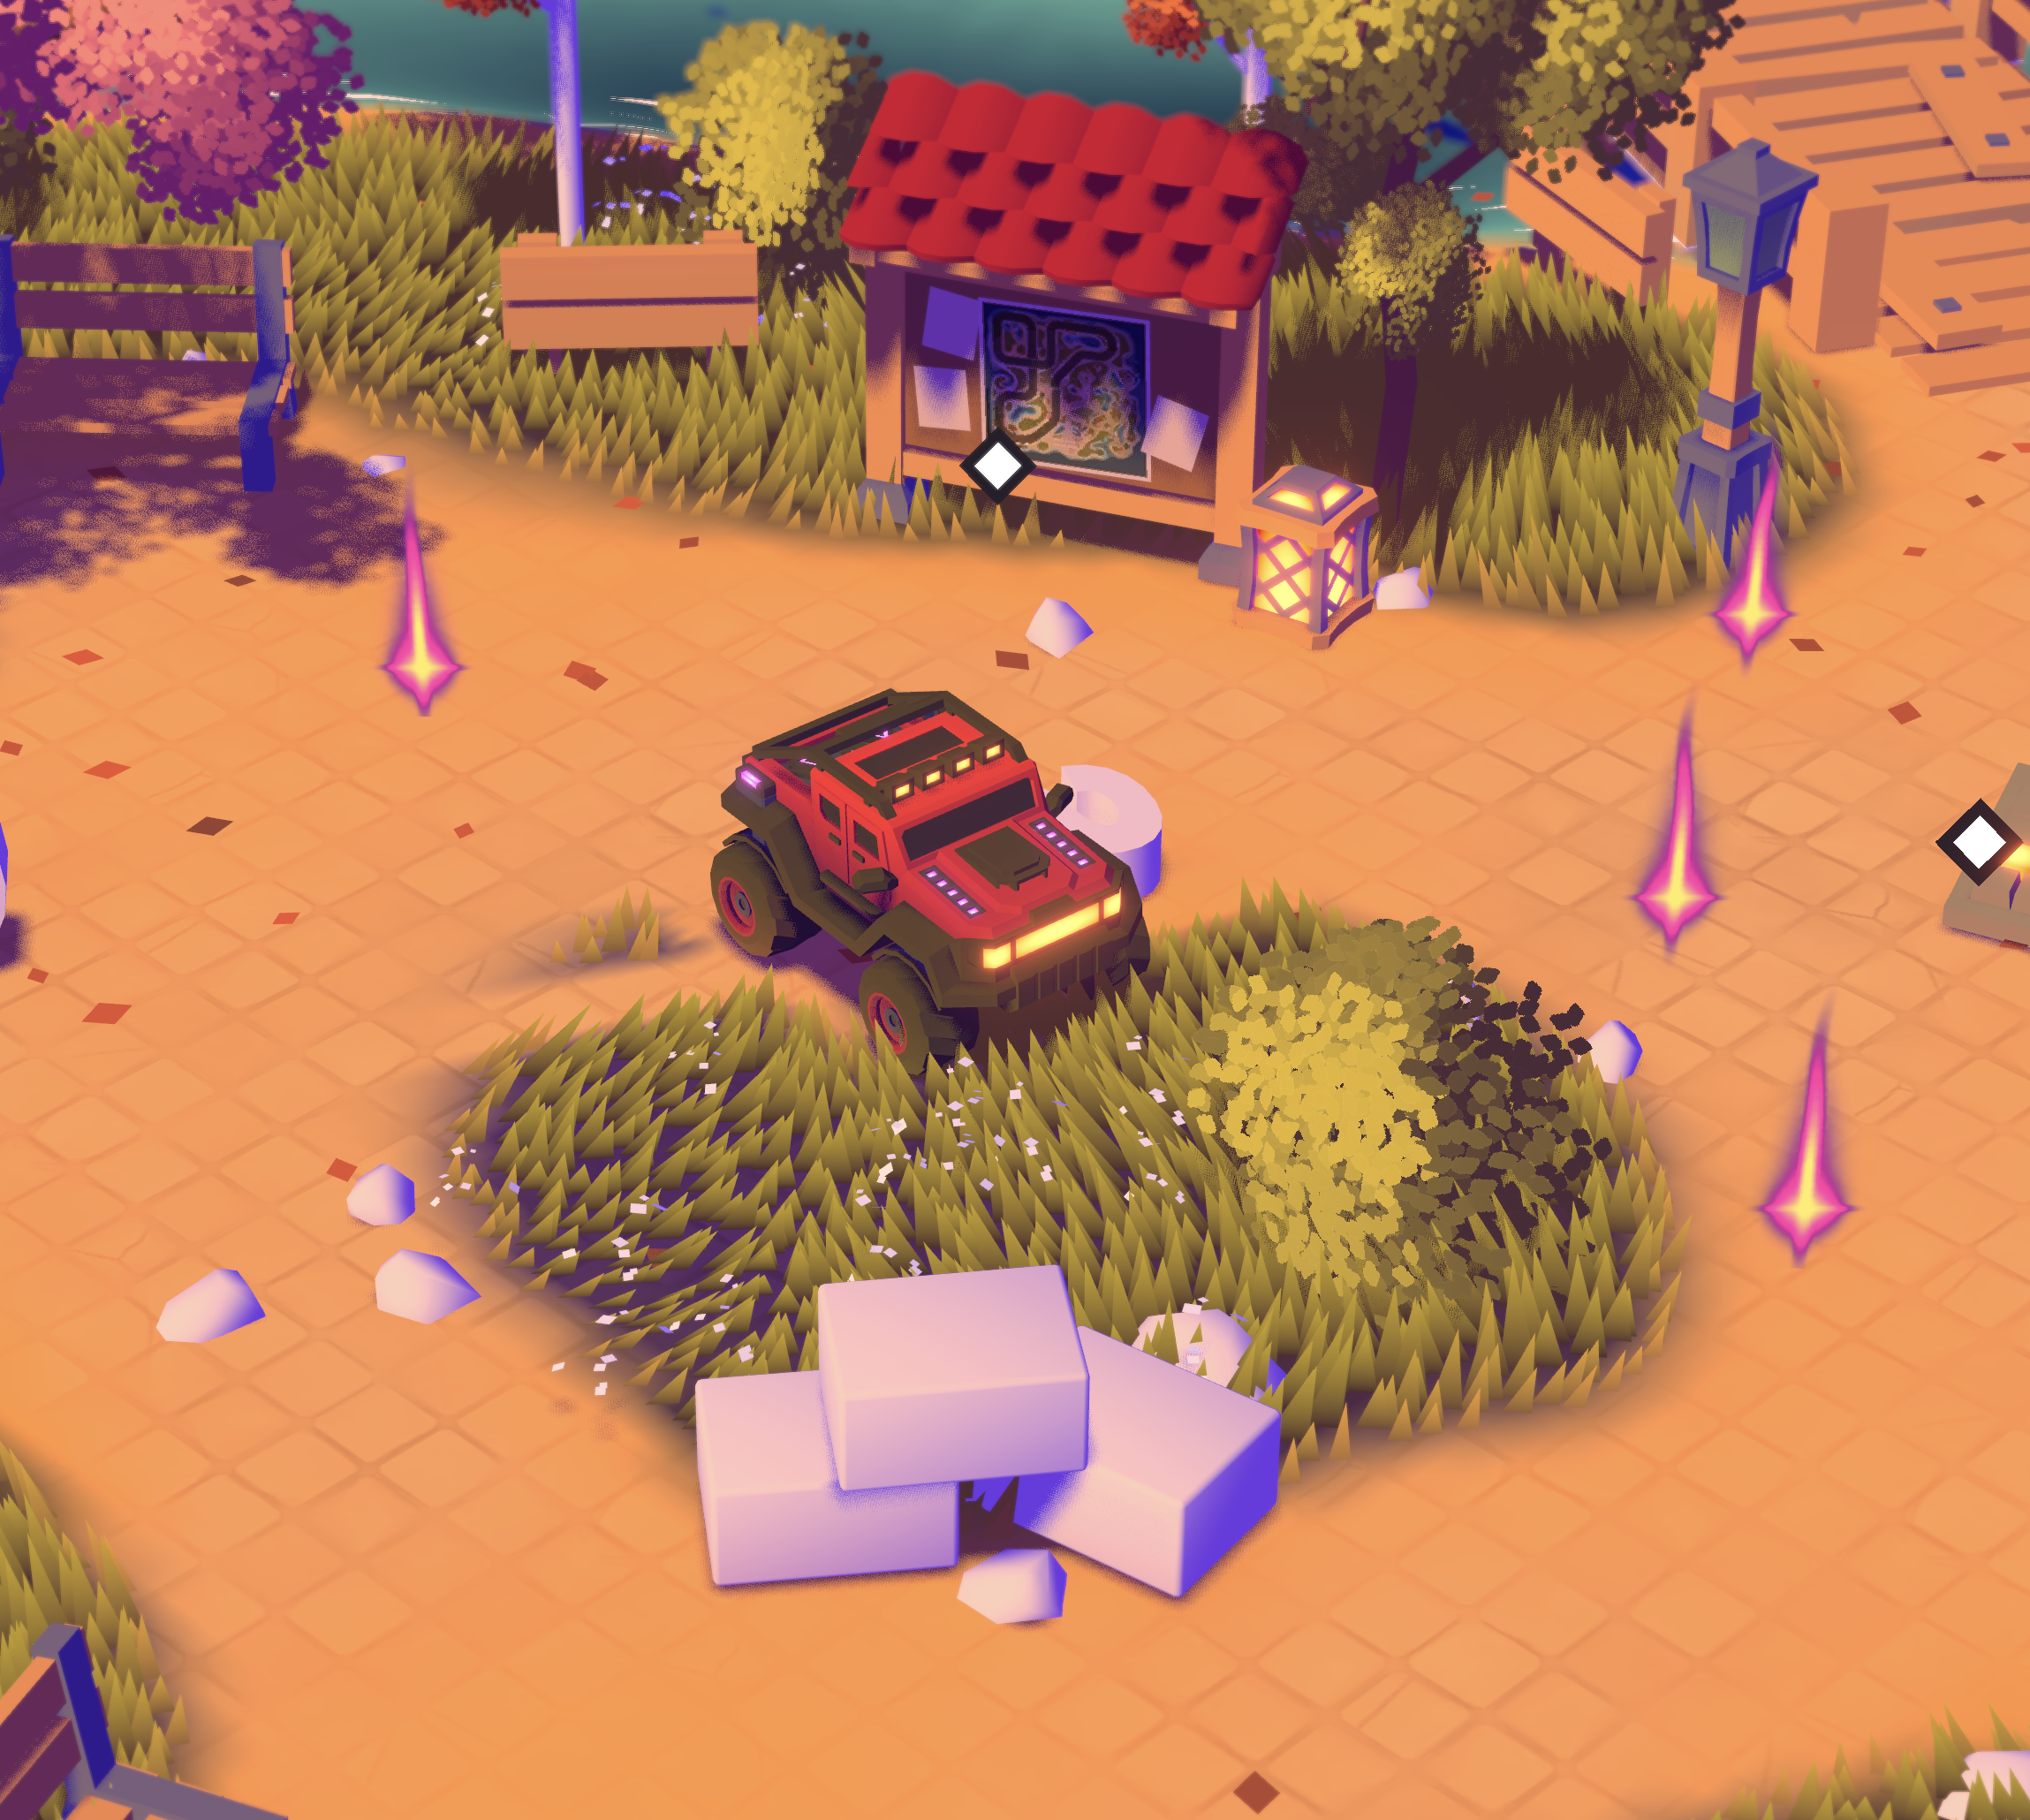
\includegraphics[width=.4\linewidth]{content/00_assets/threejs_portfolio_simon_bruno.png}
    \label{fig_threejs_portfolio_simon_bruno}
\end{figure}


Ferner lassen sich mit Three.js auch vollständig browserbasierte VR-Anwendungen auf Basis der WebXR-Technologie realisieren. Die primäre Programmiersprache des Frameworks ist JavaScript. Alternativ können auch statisch typisierte Sprachen wie TypeScript\footnote{\url{https://www.typescriptlang.org}} eingesetzt werden.

\subsection{Babylon.js}
Nebst Three.js zählt auch Babylon.js zu den etablierten webbasierten 3D-Frameworks. Babylon.js wurde im Jahr 2013 von Microsoft basierend auf der Programmiersprache TypeScript entwickelt. Wie Three.js unterstützt auch Babylon.js sowohl die Grafikschnittstellen WebGL als auch WebGPU. Im Gegensatz zu Three.js verfügt Babylon.js über eine integrierte Physik-Engine, einen Inspektor (siehe Abbildung \ref{fig_babylonjs_inspektor}) sowie einen UI-Editor \parencite{babylonjs_gui_editor_2025}. Diese umfangreiche Ausstattung trägt zur hohen Verbreitung des Frameworks bei, das rund 14’600 Downloads pro Woche verzeichnet \parencite{babylonjs_npm_2025}. Mit einer Downloadgrösse von 60 MB ist Babylon.js doppelt so gross wie Three.js. Auch Babylon.js stellt eine umfassende Dokumentation\footnote{\url{https://doc.babylonjs.com}} zur Verfügung. Ein wesentlicher Unterschied zu Three.js besteht jedoch im zugrunde liegenden Architekturansatz: Während Three.js einen stark modularen Aufbau verfolgt, gibt Babylon.js in vielen Bereichen eine feste Struktur für die Lösung typischer Problemstellungen vor \parencite{babylonjs_vs_threejs_2025}. Aufgrund der Apache-2.0-Open-Source-Lizenz kann das Framework ohne Einschränkungen auch für kommerzielle Anwendungen eingesetzt werden \parencite{babylonjs_lizenz_2025}.

\begin{figure}[H]
    \caption{Babylon.js Inspektor \parencite{babylonjs_inspector_2025}}
    \includegraphics[width=.4\linewidth]{content/00_assets/babylonjs_inspektor.png}
    \label{fig_babylonjs_inspektor}
\end{figure}

\subsection{Sokol}
Anders als browserbasierte Anwendungen werden native Applikationen direkt auf dem jeweiligen Betriebssystem ausgeführt und können auch ohne Internetverbindung genutzt werden. Jedes Betriebssystem verwendet dabei eine eigene Grafikschnittstelle: Unter Windows kommt primär DirectX zum Einsatz, unter Linux werden OpenGL oder Vulkan verwendet, während macOS auf die Metal-Schnittstelle setzt. Soll eine Anwendung plattformübergreifend verfügbar sein, muss sie entweder mehrfach implementiert oder entsprechend abstrahiert werden. Eine solche Abstraktion bietet das Framework Sokol\footnote{\url{https://github.com/floooh/sokol}}, das \textbf{unterschiedliche Grafikschnittstellen vereinheitlicht}. Somit kann eine Anwendung \textbf{einmalig entwickelt} und anschliessend auf mehreren Plattformen eingesetzt werden. Sokol steht unter der ZLib-Open-Source-Lizenz und kann somit uneingeschränkt auch für kommerzielle Projekte verwendet werden. Das Framework ist in der systemnahen Programmiersprache C implementiert und zeichnet sich durch eine hohe Leistungsfähigkeit sowie einen geringen Speicherbedarf aus. Zur Unterstützung der Entwicklung stellt Sokol verschiedene Werkzeuge bereit, die den Umgang mit 3D-Grafikschnittstellen erleichtern. Das Tool sokol-shdc\footnote{\url{https://github.com/floooh/sokol-tools/blob/master/docs/sokol-shdc.md}} ermöglicht beispielsweise die automatische Erzeugung von Shader-Programmen für unterschiedliche Zielplattformen (eine detailliertere Erklärung zu Shader folgt in Kapitel \ref{chap_render_pipelines}). Zusätzlich zu klassischen Betriebssystemen wird auch der Webbrowser als Zielplattform unterstützt. Hierfür wird \acrfull{Wasm} genutzt, um C-Code in eine für den Browser verständliche Form zu übersetzen. Wasm bietet den Vorteil einer geringen Dateigrösse sowie einer effizienten Ausführung. Wie Three.js verfolgt auch Sokol einen modularen Aufbau. Die einzelnen Komponenten werden als ``Single Header Libraries'' bereitgestellt, bei denen der gesamte Code in jeweils einer einzelnen Datei enthalten ist und keine externen Abhängigkeiten bestehen. Dies erleichtert die Integration in bestehende Projekte erheblich, da kein komplexes Build-System erforderlich ist. Die Dokumentation ist in Form von Quellcode-Kommentaren in den jeweiligen Header-Dateien enthalten. Ergänzend stehen verschiedene Beispielanwendungen zur Verfügung, die auch im Browser ausgeführt werden können (siehe Abbildung \ref{fig_sokol_beispiele}).

\begin{figure}[H]
    \caption{Sokol Beispiele \parencite{sokol_beispiele_2025}}
    \includegraphics[width=.6\linewidth]{content/00_assets/sokol_beispiele.png}
    \label{fig_sokol_beispiele}
\end{figure}

\subsection{Electron}
\label{chap_electron}
Bisher wurden sowohl webbasierte als auch native Frameworks thematisiert. Webbasierte Frameworks bieten gegenüber nativen Lösungen den Vorteil, dass keine Installation erforderlich ist und sie auf einem breiten Spektrum unterschiedlicher Endgeräte ausgeführt werden können. Jedoch existieren auch Einschränkungen, insbesondere beim Zugriff auf systemnahe Funktionen wie Multithreading oder das Dateisystem.

Electron\footnote{\url{https://www.electronjs.org}} ist ein Framework, das es ermöglicht, browserbasierte Anwendungen als native Desktop-Applikationen auf dem Betriebssystem auszuführen. Hierfür kombiniert Electron die Webanwendung mit einem Chromium-Browser sowie einer Node.js-Runtime zu einer eigenständigen Anwendung \parencite{electron_documentation_2025}. Dieser Ansatz führt zwar zu einem höheren Festplattenverbrauch im Vergleich zu klassisch nativen Anwendungen, ermöglicht jedoch gleichzeitig den Zugriff auf systemnahe Funktionalitäten wie Kamera und Dateisystem \parencite{electron_why_2025}. Aufgrund der MIT-Lizenz kann Electron zudem kostenfrei und ohne Einschränkungen für kommerzielle Anwendungen eingesetzt werden \parencite{electron_license_2021}.

\subsection{Tauri}
Tauri\footnote{\url{https://v2.tauri.app}} verfolgt das gleiche Ziel wie Electron. Anstelle eines Webbrowsers nutzt Tauri jedoch sogenannte ``WebViews''. Webviews sind Softwarekomponenten, die das Einbetten webbasierter Inhalte in native Anwendungen ermöglichen und auf allen gängigen Betriebssystemen verfügbar sind. Da WebViews deutlich weniger Ressourcen benötigen als vollwertige Browser, fällt der Festplattenbedarf entsprechend geringer aus. Eine auf Tauri basierende Anwendung kann auf eine Grösse von bis zu 600 KB reduziert werden. Im Vergleich zu den typischerweise 80–150 MB einer Electron-Anwendung ergibt sich dadurch eine erhebliche Einsparung. WebViews werden bereits von Unternehmen wie Microsoft in Produkten wie Microsoft Teams eingesetzt \parencite{microsoft_teams_webview_2023}. Der Zugriff auf native Betriebssystemfunktionen wird in Tauri über verschiedene Module realisiert, die in der systemnahen Programmiersprache Rust implementiert sind. Die Verwendung von WebViews bringt jedoch auch Einschränkungen mit sich. Da jedes Betriebssystem eine eigene WebView-Implementierung verwendet, können sich plattformspezifische Unterschiede im Funktionsumfang ergeben. Stehen jedoch ein geringer Speicherbedarf sowie eine ressourcenschonende Ausführung im Vordergrund, stellt Tauri eine attraktive Alternative zu Electron dar.

\section{Immersive Technologien}
Frameworks und Engines bilden die technische Grundlage für die Gestaltung ansprechender 3D-Erlebnisse. Für ein immersives Nutzungserlebnis sind sie allein jedoch nicht ausreichend. Technologien wie \acrshort{VR} und \acrshort{CAVE}-Systeme tragen wesentlich dazu bei, die Immersion zu erhöhen und das Gefühl zu vermitteln, sich unmittelbar innerhalb der virtuellen Umgebung zu befinden.

\subsection{Virtual Reality}
Bei klassischen 3D-Anwendungen interagieren Personen in der Regel über einen Bildschirm mit der Visualisierung. \acrfull{VR} verfolgt einen anderen Ansatz, bei dem anstelle des Bildschirms ein VR-Headset sowie entsprechende Controller zum Einsatz kommen (siehe Abbildung \ref{fig_vr_headset_controller}). Dadurch entsteht ein hohes Mass an Immersion. Die Controller ermöglichen die Bewegung innerhalb der virtuellen Umgebung, während das Headset eine freie Wahl der Blickrichtung erlaubt. Voraussetzung für ein immersives Erlebnis sind ausreichender Bewegungsfreiraum sowie eine korrekte Kalibrierung der eingesetzten Geräte. Webframeworks wie Three.js und Babylon.js ermöglichen es, VR-Anwendungen direkt im Browser mithilfe der WebXR-API\footnote{\url{https://immersiveweb.dev/}} umzusetzen. Somit sind VR-Anwendungen nicht ausschliesslich auf native Plattformen beschränkt, sondern können eine deutlich breitere Zielgruppe erreichen.

\begin{figure}[H]
    \caption{Person mit VR-Headset und Controller \parencite{vr_headset_controller}}
    \includegraphics[width=.3\linewidth]{content/00_assets/vr_headset_controller.jpg}
    \label{fig_vr_headset_controller}
\end{figure}

\subsection{Cave Automatic Virtual Environment}
\label{chap_cave}
Anders als bei Virtual Reality ist bei CAVE-Systemen kein Headset erforderlich. Stattdessen wird ein spezieller Raum genutzt, in dem sich Personen frei bewegen können und der mit geeigneten Projektoren sowie Rechnern ausgestattet ist. Während sich die Personen in der Raummitte befinden, wird die Visualisierung dabei auf die umgebenden Wände projiziert \parencite{cave_1992}. So entsteht der Eindruck, sich innerhalb der dargestellten Szene zu befinden. Ein wesentlicher Vorteil von CAVE-Systemen liegt in der einfachen Möglichkeit zur \textbf{Kollaboration}. Mehrere Beteiligte können sich gleichzeitig im selben Raum aufhalten und zentrale Aspekte der Visualisierung gemeinsam diskutieren (siehe Abbildung \ref{fig_cave_collaboration}). Insbesondere im Bildungsbereich sowie bei wissenschaftlichen Visualisierungen stellt dies einen erheblichen Mehrwert dar \parencite{cave_collaboration_2020}.

\begin{figure}[H]
    \caption{Kollaboration in einem CAVE-System \parencite[S. 11]{cave_collaboration_2020}}
    \includegraphics[width=.5\linewidth]{content/00_assets/cave_collaboration.png}
    \label{fig_cave_collaboration}
\end{figure}

Die Anschaffungskosten professioneller CAVE-Systeme liegen im Vergleich zu VR-Systemen deutlich höher. Nebst dem eigentlichen Raum werden mehrere Projektoren, Rechner sowie zusätzliche Hardwarekomponenten benötigt. Ferner ist eine entsprechende Software notwendig, die eine verzerrungsfreie und synchronisierte Projektion der Visualisierung auf die umgebenden Wände gewährleistet. Ein bewährter Ansatz zur Umsetzung dieser Synchronisation ist das sogenannte Master-Slave-Konzept \parencite{Flynn2014CAVE}. Dabei wird jede Wand des CAVE-Systems von einem eigenen Rechner mit angeschlossenem Projektor angesteuert, auf dem \textbf{dieselbe Visualisierung} ausgeführt wird. Ein zentraler Rechner fungiert als \textbf{Master} und gibt den zeitlichen Takt vor. Zudem übermittelt dieser relevante Synchronisationsdaten wie die Kameraposition, an die übrigen Rechner (\textbf{Slaves}). Diese visualisieren daraufhin jeweils ihren spezifischen Ausschnitt der Visualisierung in Abhängigkeit vom vorgegebenen Takt und den empfangenen Synchronisationsinformationen.

CAVE-Systeme lassen sich durch entsprechende Hardware flexibel erweitern. Beispielsweise ermöglicht der Einsatz von Head-Tracking-Hardware die dynamische Erfassung der Position im Raum, wodurch sich die Visualisierung in Echtzeit anpassen kann und so neue Blickwinkel eröffnet werden. Aufgrund der Vielzahl möglicher Erweiterungen ergeben sich entsprechend unterschiedliche Preissegmente, die von vierstelligen Beträgen bis zu hohen siebenstelligen Investitionen reichen können. Für die Planung und Inbetriebnahme solcher Systeme existieren spezialisierte Anbieter wie Inside Reality\footnote{\url{https://inside-reality.com/product/icroom}}, die zusätzlich zur notwendigen Software auch passende Hardwarelösungen sowie fachliche Expertise anbieten.